\documentclass[border=3pt]{standalone}
% Shared TikZ styles for the Ch. 3–8 diagrams (standalone PDFs); extends the Ch. 1 palette (s1_vs_llm_common.tex).
\usepackage[T1]{fontenc}
\usepackage{lmodern}
\usepackage[english]{babel}
\usepackage{amsmath,amssymb}
\usepackage{tikz}
\usetikzlibrary{shapes.geometric,shapes.misc,positioning,fit,arrows.meta,calc,backgrounds,decorations.pathreplacing,patterns}
\definecolor{ioFill}{HTML}{F1F0EC}\definecolor{ioLine}{HTML}{52514E}
\definecolor{modFill}{HTML}{E8F1FB}\definecolor{modLine}{HTML}{2A78D6}
\definecolor{decFill}{HTML}{ECE9F7}\definecolor{decLine}{HTML}{4A3AA7}
\definecolor{postFill}{HTML}{FFF6E0}\definecolor{postLine}{HTML}{EDA100}
\definecolor{okFill}{HTML}{EAF7F1}\definecolor{okLine}{HTML}{1BAF7A}
\definecolor{badFill}{HTML}{FDECEC}\definecolor{badLine}{HTML}{E34948}
\definecolor{nmFill}{HTML}{EFEAF8}\definecolor{nmLine}{HTML}{4A3AA7}
\definecolor{loopRed}{HTML}{E34948}\definecolor{clusterLine}{HTML}{9A9890}\definecolor{ink2}{HTML}{52514E}
\definecolor{orangeA}{HTML}{EB6834}
\tikzset{
  every node/.style={font=\small, align=center},
  io/.style={trapezium, trapezium left angle=72, trapezium right angle=108, trapezium stretches body,
             draw=ioLine, fill=ioFill, thick, inner sep=3pt, minimum height=2.4em},
  model/.style={rectangle, draw=modLine, fill=modFill, very thick, inner sep=4pt, minimum height=2.4em, text width=#1},
  model/.default=3.6cm,
  post/.style={rectangle, draw=postLine, fill=postFill, very thick, inner sep=4pt, minimum height=2.2em, text width=#1},
  post/.default=3.6cm,
  data/.style={cylinder, shape border rotate=90, aspect=0.18, draw=okLine, fill=okFill, very thick, inner sep=3pt, minimum height=2.6em, text width=#1},
  data/.default=2.4cm,
  decision/.style={diamond, aspect=2.1, draw=decLine, fill=decFill, very thick, inner sep=1pt},
  outcome/.style={rounded rectangle, draw=#1, thick, inner sep=4pt, minimum height=2em},
  arrow/.style={-{Latex[length=2mm]}, thick, ioLine},
  dashedarrow/.style={-{Latex[length=2mm]}, thick, ioLine, dashed},
  loop/.style={-{Latex[length=2.4mm]}, line width=1.4pt, loopRed},
  cluster/.style={draw=clusterLine, dashed, rounded corners=3pt, inner sep=7pt},
  clusterlabel/.style={font=\small\bfseries, text=ioLine},
  note/.style={font=\footnotesize, text=ink2},
  tok/.style={rectangle, draw=ioLine, fill=ioFill, thin, inner sep=2pt, minimum height=1.6em, font=\footnotesize},
  vmark/.style={rectangle, draw=orangeA, fill=postFill, thick, inner sep=2pt, minimum height=1.6em, font=\footnotesize\ttfamily},
}

\begin{document}
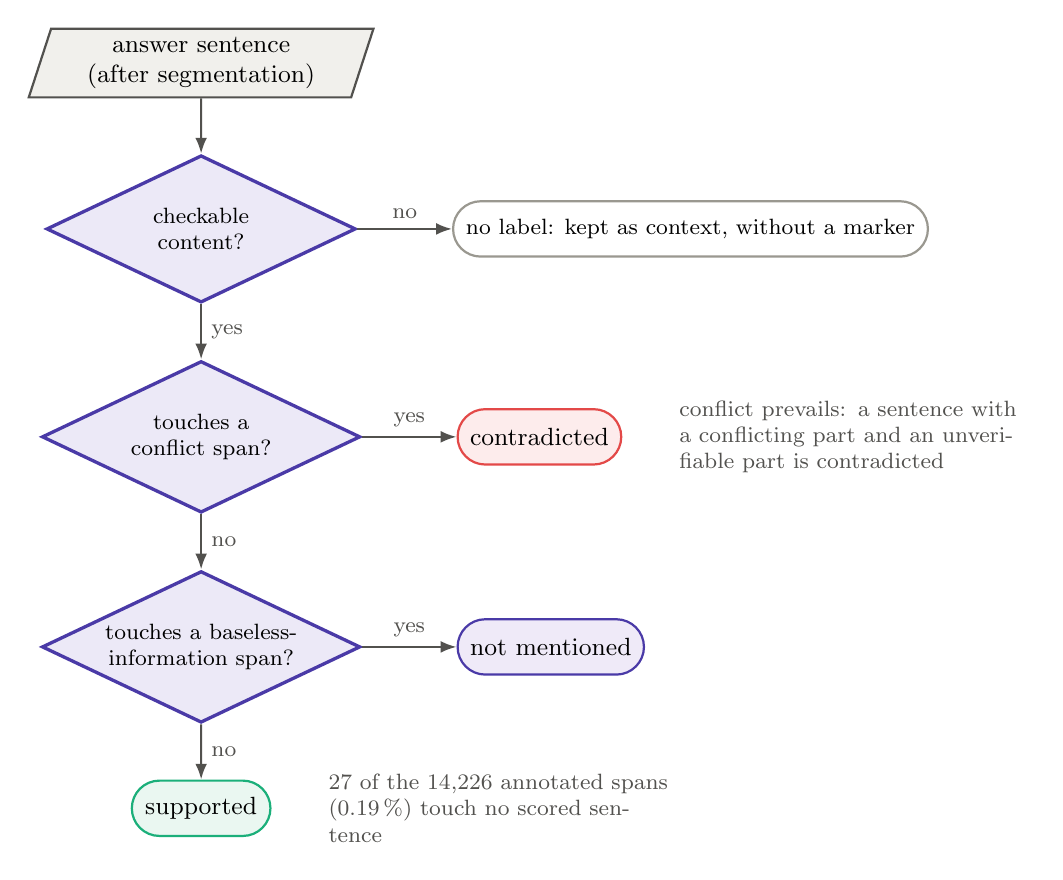
\begin{tikzpicture}[node distance=7mm]
  \node[io, text width=3.6cm] (s) {answer sentence\\(after segmentation)};
  \node[decision, below=of s, font=\footnotesize, text width=2.6cm] (d0) {checkable\\content?};
  \node[outcome=clusterLine, fill=white, right=12mm of d0, font=\footnotesize] (ctx) {no label: kept as context, without a marker};
  \node[decision, below=of d0, font=\footnotesize, text width=2.6cm] (d1) {touches a\\conflict span?};
  \node[outcome=badLine, fill=badFill, right=12mm of d1] (con) {contradicted};
  \node[decision, below=of d1, font=\footnotesize, text width=2.6cm] (d2) {touches a baseless-\\information span?};
  \node[outcome=nmLine, fill=nmFill, right=12mm of d2] (nm) {not mentioned};
  \node[outcome=okLine, fill=okFill, below=of d2] (sup) {supported};
  \draw[arrow] (s) -- (d0);
  \draw[arrow] (d0) -- node[above, font=\footnotesize] {no} (ctx);
  \draw[arrow] (d0) -- node[right, font=\footnotesize] {yes} (d1);
  \draw[arrow] (d1) -- node[above, font=\footnotesize] {yes} (con);
  \draw[arrow] (d1) -- node[right, font=\footnotesize] {no} (d2);
  \draw[arrow] (d2) -- node[above, font=\footnotesize] {yes} (nm);
  \draw[arrow] (d2) -- node[right, font=\footnotesize] {no} (sup);
  \node[note, right=6mm of con, text width=4.4cm, align=left] {conflict prevails: a sentence with a conflicting part and an unverifiable part is contradicted};
  \node[note, right=6mm of sup, text width=4.4cm, align=left] {27 of the 14{,}226 annotated spans (0.19\,\%) touch no scored sentence};
\end{tikzpicture}
\end{document}
